\chapter{基于集中平台的iBGP系统结构}
\label{cha:china}


\section{本章引言}
可扩展问题是互联网iBGP协议的重要问题,随着网络规模和需求的不断增加,大多数自治系统已经不采用传统的Full-mesh的iBGP连接结构,而是使用配置比较方便、技术比较成熟的路由反射。现有的解决iBGP可扩展问题的思路可分为两种:分布式路由体系结构、集中式路由体系结构。分布式路由体系结构下的相关研究主要有路由反射和AS联邦,其解决了iBGP的可扩展问题,但是带来了新的问题,比如:非最优出口、转发环路、路由震荡。而集中式路由体系结构的相关研究主要有SoftRouter、RCP、RFCP三种代表性方案,这三种方案解决了iBGP的可扩展问题,但也分别存在集中平台本身的可扩展性差、路由存储冗余重复、未优化的传统路由计算方式等等问题。

本文基于数据平面和控制平面分离的思想,提出了基于集中平台的iBGP系统结构,将自治系统内部的路由存储、策略管理、路由计算以及路由转发交换功能合理划分为集中平台和自治系统内边界路由器上执行的两部分。该基于集中平台的iBGP系统结构处理路由信息的基本流程为:
\begin{itemize}
  \item 自治系统内的边界路由器收到路由信息,通过iBGP协议将从eBGP经过收到的路由信息发送到集中平台;
  \item 集中平台执行路由信息存入路由信息表Adj-RIB-In、将路由信息进行入站过滤后存入Loc-RIB、为每台自治系统内的边界路由器计算出最优路由、进行出站过滤等操作;
  \item 集中平台上将过滤后的最优路由传输给域内的每台边界路由器,边界路由器将收到的路由信息通过eBGP连接宣告出去。
\end{itemize}

集中式路由体系结构下,路由存储、策略管理、路由计算等存在很多优化空间。本文提出的基于集中平台的iBGP系统,不仅解决了iBGP存在的可扩展问题,而且对自治系统内BGP的路由存储和路由计算进行了优化。

本章首先提出基于集中平台的iBGP系统架构,之后对系统中的两个主要模块增量路由存储、复式路由计算进行详细的介绍,最后主要从解决iBGP可扩展问题、与分布式路由体系结构方案的对比、与集中式路由体系结构方案的这三个方面对基于集中平台的iBGP系统进行定性的分析。



\begin{figure}
  \centering
  % Requires \usepackage{graphicx}
  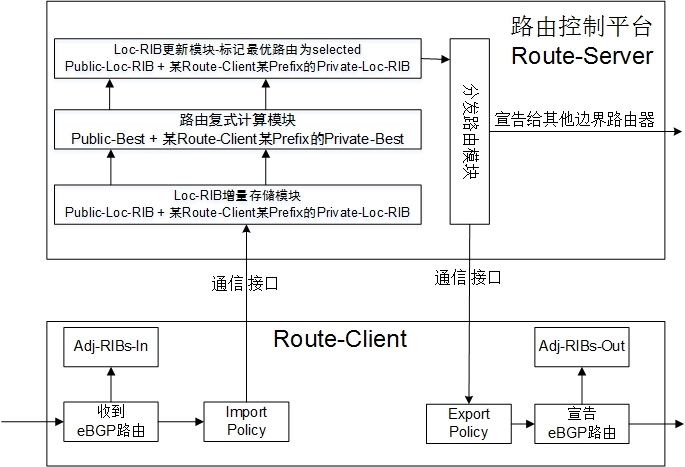
\includegraphics[width=\textwidth]{rscp-ibgp}
  \caption{RSCP-iBGP系统架构图}
  \label{fig:rscp-ibgp}
\end{figure}

\section{新型iBGP路由系统}
本文提出的自治系统内部的基于集中平台的iBGP新架构命名为RSCP-iBGP(Route Server Control Platform iBGP)。RSCP-iBGP基本思想是将自治系统内边界路由器的控制平面和数据平面分离,将边界网关协议BGP中的路由计算、路由存储、路由策略从边界路由器中剥离出来,交由独立的、且逻辑比较集中的运行在路由控制平台的Route-Server执行,而自治系统内部的普通边界路由器作为Route-Client对路由信息进行接收转发等操作。RSCP-iBGP系统如图\ref{fig:rscp-ibgp},这个系统运行在自治系统内部,主要包含三部分:自治系统内部的路由控制平台(Route-Server),自治系统内部的多台边界路由器(Route-Client),以及自治系统内部边界路由器与路由控制平台的标准通信接口(iBGP协议):
\begin{itemize}
  \item 通信协议使用iBGP协议,来传输BGP路由信息;
  \item 路由控制平台上运行1台Route-Server进行集中式的路由存储、策略管理、路由计算。当Route-Server收集路由模块,收集到自治系统内部边界路由器Route-Client-Ri发来的更新路由消息,Route-Server现将该路由加入Adj-RIBs-In表,之后该路由经过Route-Client-Ri的入站策略后进入Loc-RIB增量存储模块,存储经过入站策略的路由信息,将Loc-RIB表以及IGPcost值输入路由复式计算模块,得到自治系统每台边界路由的针对该前缀的最优路由,之后在路由集中控制平台上分别经过每台边界路由器的出站策略,更新每台边界路由器的Adj-RIBs-Out表,将其结果输入到分发路由模块,分发路由模块则分别将经过出站策略的该前缀的最优路由传输给自治系统内的每台边界路由;
  \item 自治系统内部的边界路由器Route-Cleint:当收到eBGP路由时,将其通过iBGP协议发送给路由控制平台上的Route-Server;当收到路由控制平台上的Route-Server发来的iBGP路由时,Route-Client将其宣告给自己的所有eBGP邻居。
\end{itemize}

\section{系统模块介绍}
\subsection{路由存储}
传统的运行BGP协议的自治系统内的边界路由器,在路由信息的处理过程中,需要使用三种RIB表,分别是Adj-RIBs-In、Loc-RIB、Adj-RIBs-Out表。在RSCP-iBGP的新架构中,仍需要存储Loc-RIB表,Adj-RIBs-In和Adj-RIBs-Out根据需要进行存储。
\subsubsection{Adj-RIBs-In}
一般运行BGP协议的路由器默认不存储从邻居获得的所有未经入站策略的路由信息,即默认不存储Adj-RIBs-In。如果路由器想要存储从某个BGP邻居收到的所有未经入站策略的路由信息,则需要通过配置文件进行配置,对应的语句为:neighbor [ip-address] soft-reconfiguration inbound,该语句告诉BGP进程保存从指定邻居那里获得的所有更新。


假设自治系统有N台边界路由器Route-Client,Route-Server路由器与这N台Route-Client分别建立N个iBGP连接,如果Route-Server在某个iBGP连接的neighbor配置里面设置了保存收到的所有更新,则Route-Server存储从对应的Route-Client收到的所有未经入站策略的原始路由信息Adj-RIB-In。通过语句show ip bgp neighbors [ip-address] received-routes可以查看Adj-RIB-In。


\subsubsection{Loc-RIB增量存储模块}

\begin{figure}
  \centering
  % Requires \usepackage{graphicx}
  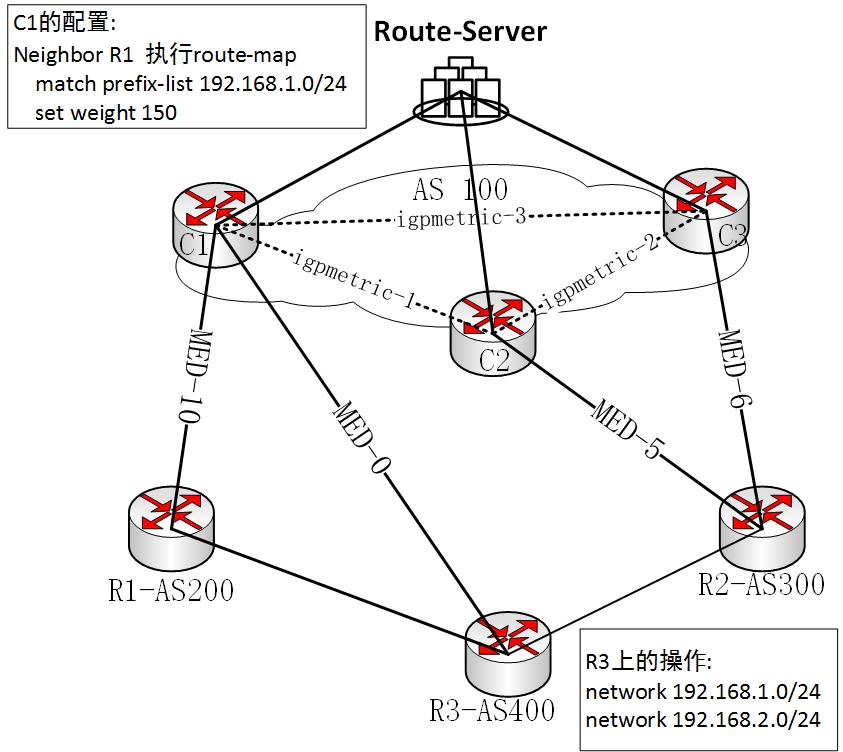
\includegraphics[width=0.75\textwidth]{rscp-example1}
  \caption{Loc-RIB增量存储案例使用的网络拓扑图}
  \label{fig:rscp-example1}
\end{figure}

传统网络中,自治系统的边界路由器收到从eBGP邻居传来的更新路由信息,该边界路由器会将该路由信息经过入站策略后更新到Loc-RIB表,选择最优路由宣告给其iBGP邻居。早期自治系统内的边界路由器建立Full-mesh的iBGP连接,以此来使得外界的路由信息传输到自治系统内部的每台边界路由器。路由经过入站策略后,可能传输到每台边界路由器会有所差异,但大部分前缀在大部分边界路由器上的Loc-RIB表的路由信息都基本相同,入站策略和出站策略主要用于eBGP路由,传统的iBGP策略大多仅配置next-hop-self。根据BGP协议的特性以及网络中路由表的存储实现,本文提出了Loc-RIB增量存储的概念。

综合本文第二章对BGP的路由策略、路由计算的综述,我们会发现对于特定的前缀,在自治系统内的决定每台边界路由器与其他边界路由器最优路由不同的主要原因在2个路由属性Weight和IGPcost:Weight路由属性仅本地路由器有效,不传输给其他的边界路由器;不同边界路由器到其他边界路由器的IGPcost并不相同。仅从路由存储的角度考虑,可以在路由控制平台上的Route-Server中存储一份Public-Loc-RIB,以及在每个iBGP的对等体连接进程中,存储曾配置过Weight值的Prefix的所有路由表项(因为Weight仅在本地路由器有效,并不会影响其他边界路由器的选路)。Loc-RIB增量存储中增量的含义为,将每台边界路由器特有的路由信息增量存储,为了便于该边界路由器前缀最优路由的计算,将该边界路由器可能受到Weight值影响的前缀的所有路由增量存储。



\begin{table}[h]
	\centering
	\caption{Route-Server的Public-Loc-RIB数据}
    \label{tab:weight-example}
	\begin{tabular}{|c|c|c|c|c|c|c|}
		\hline
		network & next-hop & metric & LocPrf & Weight & Path & ebgp-next-hop \\ \hline
		192.168.1.0 & C1 & 0 & &  &400,i & R3 \\ \hline
        192.168.1.0 & C1 & 10 & &  &200,400,i & R1 \\ \hline
        192.168.1.0 & C2 & 5 & &  &300,400,i & R2 \\ \hline
        192.168.1.0 & C3 & 6 & &  &300,400,i & R2 \\ \hline
        192.168.2.0 & C1 & 0 & &  &400,i & R3 \\ \hline
        192.168.2.0 & C1 & 10 & &  &200,400,i & R1 \\ \hline
        192.168.2.0 & C2 & 5 & &  &300,400,i & R2 \\ \hline
        192.168.2.0 & C3 & 6 & &  &300,400,i & R2 \\ \hline
	\end{tabular}
\end{table}

在如图\ref{fig:rscp-ibgp}的拓扑中,ASN(Autonomous System Number,自治系统号)为100的自治系统在部署RSCP-iBGP系统的条件下,在Route-Server中Loc-RIB采用增量存储的方案。AS100中有3台Route-Client作为边界路由器,分别命名为C1、C2、C3。Route-Server存储了C1、C2、C3的路由策略,在集中的路由控制平台上部署了C1的入站策略(C1从R1收到的前缀为192.168.1.0/24的路由将其Weight设置为150)。



\begin{table}[h]
	\centering
	\caption{C1的Pravite-Loc-RIB数据}
    \label{tab:c1-loc-rib}
	\begin{tabular}{|c|c|c|c|c|c|c|}
		\hline
		network & next-hop & metric & LocPrf & Weight & Path & ebgp-next-hop \\ \hline
		192.168.1.0 & C1 & 0 & &  &400,i & R3 \\ \hline
        192.168.1.0 & C1 & 10 & & 150 &200,400,i & R1 \\ \hline
        192.168.1.0 & C2 & 5 & &  &300,400,i & R2 \\ \hline
        192.168.1.0 & C3 & 6 & &  &300,400,i & R2 \\ \hline
	\end{tabular}
\end{table}

当R3向外宣告两条路由192.16.1.0/24和192.168.2.0/24,Route-Server收到了C1转发过来的路由信息,其存储的Public-Loc-RIB如表\ref{tab:weight-example}。因为前缀为192.168.1.0/24的通过C1传输到集中的路由控制平台的两条路由,均需经过C1的入站策略,C1传输过来的ebgp-next-hop为从R1接收到前缀为192.168.1.0/24的路由经过入站策略路由的Weight值被重设为150,其操作可能影响之后的路由决策,则C1需要存储192.168.1.0/24的所有路由,其存储的Private-Loc-RIB如表\ref{tab:c1-loc-rib}。


从表\ref{tab:weight-example}、表\ref{tab:c1-loc-rib}可以看出,Loc-RIB的增量更新方案对于减少Loc-RIB表的存储非常有效。如果自治系统内有N台边界路由器,则Route-Server仅需存储1张Loc-RIB表,加m条单独的路由,其占用存储空间的大小直接下降了一个数量级。


\subsubsection{Adj-RIBs-Out}
一般运行BGP协议的路由器默认不存储经过出站策略准备宣告给邻居的路由信息,即默认不存储Adj-RIBs-Out。如果路由器想要存储经过出站策略准备宣告给邻居的路由信息,则需要通过配置文件进行配置,对应的语句为:neighbor [ip-address] soft-reconfiguration outbound,该语句告诉BGP进程保存向指定邻居那里宣告的所有更新。


假设自治系统有N台边界路由器Route-Client,Route-Server路由器与这N台Route-Client分别建立N个iBGP连接,如果Route-Server在某个iBGP连接的neighbor配置里面设置了保存向外宣告的所有更新,则Route-Server存储从对应的Route-Client宣告给邻居的所有路由信息。通过语句show ip bgp neighbors [ip-address] advertised-routes可以查看Adj-RIB-Out。


\subsection{路由计算}
\section{理论分析}
\subsection{解决iBGP可扩展问题}
假设某自治系统有N台边界路由器,在传统Full-mesh的iBGP结构中,域内自治系统需要建立N(N-1)/2数量的BGP连接。该自治系统的拓扑结构对应到本文的RSCP-iBGP系统结构,自制系统内的有N台Route-client边界路由器用于接受转发其他自治系统传输过来的路由、1台或者多台运行在路由控制平台的Route-Server用于路由存储和路由计算等操作,N台Route-Client与1台Route-Server建立N个扩展的iBGP连接来传输BGP路由信息,则该基于集中平台的iBGP新架构解决了iBGP协议可扩展性差的问题。


\subsection{与分布式路由体系结构方案的对比}
\subsection{与集中式路由体系结构方案的对比}
\subsection{总结}

\section{本章小结}
总结